\documentclass[professionalfont]{beamer}

\usepackage[T1]{fontenc}
\usepackage{amsmath}
\usepackage{graphicx}
\graphicspath{{figures/}}
\usepackage{tikz}

% usage: \tikzpic{<x percent>}{<y percent>}{<image size>}{<image name>}
\newcommand*{\tikzpic}[4]{%
\begin{tikzpicture}[remember picture,overlay]
\node at (current page.south west) [xshift=#1\paperwidth,yshift=#2\paperheight] {\includegraphics[width=#3\linewidth]{#4}};
\end{tikzpicture}%
}

\title[Anisotropic \texttt{fdaPDE}]{Estimation of anisotropy in a spatial field in \texttt{fdaPDE} package}
\author[S. Souque \& T. Kletti]{\underline{Samuel \textsc{Souque}}, \underline{Till \textsc{Kletti}}\\
{\small \href{mailto:samuel.souque@mail.polimi.it}{\nolinkurl{samuel.souque@mail.polimi.it}}}, \\{\small \href{mailto:tillalexander.kletti@mail.polimi.it}{\nolinkurl{tillalexander.kletti@mail.polimi.it}}}}
\date[MI, today]{Milano, \today}
\institute[POLIMI]{Politecnico di Milano}

\usetheme{POLIMI}

\usepackage{lmodern}
\usepackage[latin1]{inputenc}
\usepackage[T1]{fontenc}
\usepackage[english]{babel}


%%%%%%%%%%%%%%%%%%%% T E X T E %%%%%%%%%%%%%%%%%%%%%%

% package qui permettent d'utiliser tout un tas de symboles math?matiques
\usepackage{amsmath}
\numberwithin{equation}{section}

\usepackage{amssymb}
\usepackage{empheq}
%\usepackage{mathrsfs}
\usepackage[squaren,Gray]{SIunits} %Unit�s SI

% Polices
%\usepackage{mathpazo} %Police styl�e de J�r�my Omer
%\usepackage{txfonts} %autre police styl�e, s'approche du style de word
%\usepackage{libertine}

% permet d'?crire des caract?res chinois
%\usepackage{CJKutf8}
%Utiliser le pinyin
%\usepackage{pinyin}

% package qui permettent de personaliser les puces des listes
\usepackage{enumerate}
\usepackage{enumitem} % pour utiliser description

% package qui permettent d'introduire de la couleur
\usepackage{color}
\definecolor{mygreen}{rgb}{0,0.6,0}
\definecolor{mygray}{rgb}{0.5,0.5,0.5}
\definecolor{mymauve}{rgb}{0.58,0,0.82}

\usepackage{xspace}
% permet l'affichage de l'heure courante
%\usepackage{datetime}

%pour pouvoir barrer avec \cancel{}
%\usepackage{cancel}

%pour la fonction indicatrice 1
%\usepackage{dsfont}

%pour utiliser le symbole euro par \euro
\usepackage{eurosym}

%afficher des nombres en mode texte
\usepackage{numprint}

%Capitale grande en d�but de paraghraphe
%\usepackage{lettrine}


%%%%%%%%%%%%%%%%%%%% F I G U R E S %%%%%%%%%%%%%%%%%%%%%%

% package qui permettent d'inclure des graphiques
\usepackage{graphicx}
\numberwithin{figure}{section}

%Pour utiliser des sous-figures
\usepackage{subcaption}

%Pour utiliser [H] pour le placement des figures
\usepackage{float}

%figure entour�e de texte
\usepackage{wrapfig}
% \begin{wrapfigure}{L}{0.4\textwidth}

%Keep figures in section
\usepackage[section]{placeins}
% \FloatBarrier % stops floats from descending further

% Pour des r�f�rences styl�es
%\usepackage{varioref}
%\usepackage[german]{fancyref} % dispo seulement en allemand
\usepackage[linkcolor=black,
						urlcolor=black,
						colorlinks=true,
						citecolor=mygreen]{hyperref}% package qui cr�er des liens dynamiques dans un fichier pdf � partir de tout �l�ment tagg� 
%\usepackage{cleveref}


%%%%%%%%%%%%%%%%%%%% D E S S I N %%%%%%%%%%%%%%%%%%%%%%

%pour dessiner des graphes de fonctions
\usepackage{pgfplots}

%pour plein de commandes de dession
\usepackage{tikz}
\usetikzlibrary{decorations.pathreplacing,calligraphy}

%%%%%%%%%%%%%%%%%%%% H E A D E R et F O O T E R %%%%%%%%%%%%%%%%%%%%%%

\usepackage{fancyhdr}
%\fancyfoot{}
\fancyfoot[LE,RO]{\thepage}


%%%%%%%%%%%%%%%%%%%%%% D I V E R S %%%%%%%%%%%%%%%%%%%%%%%%%%

%Bibliographie
\usepackage[backend=bibtex,sorting=ynt]{biblatex}%sorting=none pour avoir les r�f�rences selon d'ordre d'apparition dans le texte
% sorting=ynt		backend=biber,

%pour que les textes en Verbatim soient encadr�s
%\usepackage{fancyvrb}

% Mettre en forme son texte en plusieurs colonnes
%\usepackage{multicol}

%pour manipuler les compteurs avec par exemple \counterwithin{figure}{section}
\usepackage{chngcntr}

%pour importer des sections
\usepackage{import}

%Appendices
\usepackage[title,toc,page,header]{appendix}
\renewcommand{\appendixtocname}{Tables des Annexes}
\renewcommand{\appendixpagename}{Annexes}

%\usepackage{couvresumesPFE} % utilisation du package pfe.sty pour cr�er la couverture et la page de r�sum�s en fran�ais et en anglais


%%%%%%%%%%%%%%%%%%% C O D E %%%%%%%%%%%%%%%%%%%%%%%

% Pour �crire du pseudo-code
%\usepackage{algorithm2e}
%\usepackage{algorithmic}
\usepackage{algorithm}
\usepackage{algpseudocode}
%\listofalgorithms % commande pour lister les algorithmes

%pour ins�rer du code
\usepackage{listings}
\usepackage{listingsutf8}
%\usepackage{inconsolata}
\lstdefinestyle{CodeR}{ %
  backgroundcolor=\color{white},
  basicstyle=\footnotesize,
  breakatwhitespace=false
  breaklines=true,
  captionpos=b,
  commentstyle=\color{mygreen},
  deletekeywords={...},
  escapeinside={Ratus}{Chiffon},
  extendedchars=true,
  frame=single,
  keepspaces=true,
  keywordstyle=\color{blue},
  language=R,
  otherkeywords={*,...},
  numbers=left,
  numbersep=5pt,
  numberstyle=\tiny\color{mygray},
  rulecolor=\color{black},
  showspaces=false,
  showstringspaces=false,
  showtabs=false,
  stepnumber=1,
  stringstyle=\color{mymauve},
  tabsize=4,
  title=\lstname
}
\lstdefinestyle{CodeMATLAB}{ %
  backgroundcolor=\color{white},
  basicstyle=\footnotesize,
  breakatwhitespace=false
  breaklines=true,
  captionpos=b,
  commentstyle=\color{mygreen},
  deletekeywords={...},
  escapeinside={James}{Ledoux},
  extendedchars=true,
  frame=single,
  keepspaces=true,
  keywordstyle=\color{blue},
  language=MATLAB,
  otherkeywords={*,...},
  numbers=left,
  numbersep=5pt,
  numberstyle=\tiny\color{mygray},
  rulecolor=\color{black},
  showspaces=false,
  showstringspaces=false,
  showtabs=false,
  stepnumber=1,
  stringstyle=\color{mymauve},
  tabsize=4,
  title=%\lstname
}
\lstset{style=CodeMATLAB}


% Ensemble et op�rateur avec un barre pr�c�dent le symbole
\newcommand{\E}{\mathbb{E}}
\renewcommand{\P}{\mathbb{P}}
\newcommand{\N}{\mathbb{N}}
\newcommand{\Q}{\mathbb{Q}}
\newcommand{\Z}{\mathbb{Z}}
\newcommand{\R}{\mathbb{R}}
\newcommand{\V}{\mathbb{V}}
\newcommand{\1}{\mathds{1}}%n�cc�cite le package dsfont

% Lettres calligaphiques
\newcommand{\cA}{\mathcal{A}}
\newcommand{\cU}{\mathcal{U}}
\newcommand{\cN}{\mathcal{N}}
\newcommand{\cE}{\mathcal{E}}
\newcommand{\cC}{\mathcal{C}}
\newcommand{\cI}{\mathcal{I}}
\newcommand{\cO}{\mathcal{O}}

% Utilisation du diff�rentiel d
\renewcommand{\d}[1]{\,\ensuremath{\operatorname{d}\!{#1}}}

% D?finition des envrionement de type ?nonc?s num?rot?s simplement
\newtheorem{theo}{Th?or?me}
\newtheorem{rema}{Remarque}
\newtheorem{exem}{Exemple}
\newtheorem{defi}{D?finition}
\newtheorem{exer}{Exercice}
\newtheorem{prop}{Proposition}
\newtheorem{code}{Code}

% D?finition des m?mes envrionements de type ?nonc?s num?rot?s mais avec l'ajout pr?alable de la section
\newtheorem{adef}{D?finition}[section]
\newtheorem{apro}{Proposition}[section]
\newtheorem{athe}{Th?or?me}[section]
\newtheorem{aexe}{Exercice}[section]
\newtheorem{aexem}{Exemple}[section]
\newtheorem{arem}{Commentaire}[section]

% D?finition d'un environement qui utilise le m?me compteur que l'environnement athe
\newtheorem{thm}[athe]{M?me compteur que Th?or?me }

% D?finition d'une commande qui met une boite blanche en but de ligne
%\newcommand{\fdem}{\hspace*{\fill}~$\Box$\par\endtrivlist\unskip}

% D?finition d'un nouvelle environnement avec un argument. La fin de l'environnement est marqu? par le symbole g?n?r? par la commande \fdem
%\newenvironment{proof}[1]{\textit{Preuve#1.\,}}{\fdem}

% R�f�rencement fain�ant des figures
%\newcommand{\tref}[1]{\textsc{Fig.} \ref{#1}}

%indiquer la source d'une figure avec \source{La source}
%\newcommand{\source}[1]{\vspace{-10pt} \caption*{\footnotesize \textbf{Source:} {#1}} }


\begin{document}
\begin{frame}[plain]
\titlepage
\end{frame}

\begin{frame}{Table of contents}
\tableofcontents
\end{frame}

\section{Introduction}

\begin{frame}{Introduction}
\begin{block}{The Problem}
Given samples from a spatial field, characterize the anisotropy of the field.
\end{block}
\begin{block}{Mathematical formulation}
	We seek to minimize
	\begin{equation}
		J_\lambda(\hat{f},K) = \sum_{i=1}^N (\hat{f}(x_i)-f(x_i))^2 + \lambda\int_\Omega \nabla(K\nabla\hat{f}(x)) \d{x}
	\end{equation}
	with respect to the estimated field $\hat{f}$, the anisotropy matrix $K$ and the regularization coefficient $\lambda$.
\end{block}
% That is, we seek the anisotropy K
\end{frame}

\section{Method}

\begin{frame}{The algorithm}
	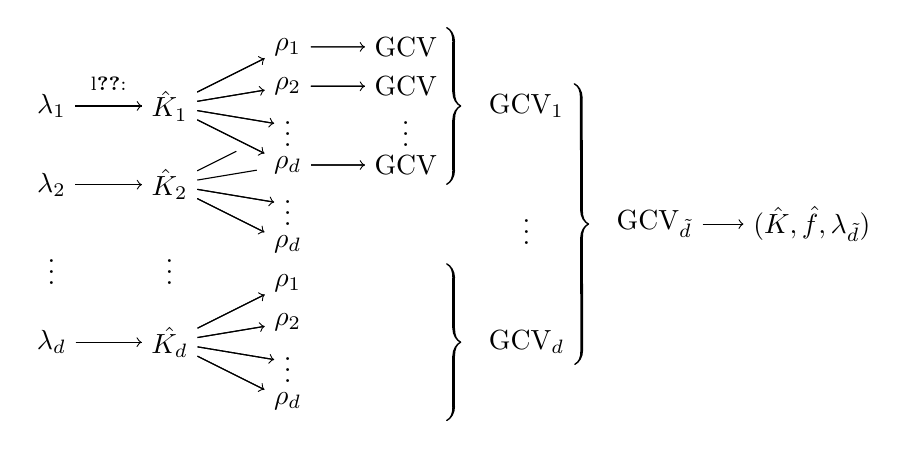
\begin{tikzpicture}[node distance=1cm]
\tikzstyle{level 1}=[sibling distance=5mm]
	\node (l1){$\lambda_1$}
		child[grow=right]{node (K1){$\hat{K}_1$}
			child{node (rhod){$\rho_d$}
				child{node (GCVd){GCV}} }
			child{node (rhodot){$\vdots$}
				child{node[draw=none] (GCVdot){$\vdots$} edge from parent[draw=none] } }
			child{node (rho2){$\rho_2$}
				child{node (GCV2){GCV}} }
			child{node (rho1){$\rho_1$}
				child{node (GCV1){GCV}} }
};
	\draw[->] (l1) edge node [midway, above = 2pt]{ \scriptsize{l\ref{lst:K}:} } (K1) ;
	\draw[->] (K1) edge (rho1);
	\draw[->] (K1) edge (rho2);
	\draw[->] (K1) edge (rhodot);
	\draw[->] (K1) edge (rhod);
	\draw[->] (rho1) edge (GCV1);
	\draw[->] (rho2) edge (GCV2);
	\draw[->] (rhod) edge (GCVd);

	\draw[decoration={calligraphic brace,amplitude=5pt}, decorate, line width=1pt]
		(GCV1.north east) -- (GCVd.south east) node [midway,xshift=0.4cm,right] (GCVa){$\text{GCV}_1$};

	
	\node[below of=l1] (l2){$\lambda_2$}
		child[grow=right]{node (K2){$\hat{K}_2$}
			child{node (rhod2){$\rho_d$} }
			child{node (rhodot2){$\vdots$} }
			child{node (rho22){\phantom{$\rho_2$}} edge from parent[draw=none]}
			child{node (rho12){\phantom{$\rho_1$}} edge from parent[draw=none]}
};
	\draw[->] (l2) edge (K2);
	\draw[shorten >=0.4cm] (K2) edge (rho12);
	\draw[shorten >=0.1cm] (K2) edge (rho22);
	\draw[->] (K2) edge (rhodot2);
	\draw[->] (K2) edge (rhod2);
%	\draw[->] (rho12) edge (GCV12);
%	\draw[->] (rho22) edge (GCV22);
%	\draw[->] (rhod2) edge (GCVd2);


	\node[below of=l2] (ldot){$\vdots$}
		child[grow=right]{node (Kdot){$\vdots$} edge from parent[draw=none]};
	\node[below of=ldot] (ld){$\lambda_d$}
		child[grow=right]{node (Kd){$\hat{K_d}$}
			child{node (rhodd){$\rho_d$}
				child{node (GCVdd){\phantom{GCV}} edge from parent[draw=none] } }
			child{node (rhodotd){$\vdots$}
				child{node (GCVdotd){\phantom{$\vdots$}} edge from parent[draw=none] } }
			child{node (rho2d){$\rho_2$}
				child{node (GCV2d){\phantom{GCV}} edge from parent[draw=none] } }
			child{node (rho1d){$\rho_1$}
				child{node (GCV1d){\phantom{GCV}} edge from parent[draw=none] } }
 };
	\draw[->] (ld) edge (Kd);
	\draw[->] (Kd) edge (rho1d);
	\draw[->] (Kd) edge (rho2d);
	\draw[->] (Kd) edge (rhodotd);
	\draw[->] (Kd) edge (rhodd);

	\draw[decoration={calligraphic brace,amplitude=5pt}, decorate, line width=1pt]
		(GCV1d.north east) -- (GCVdd.south east) node [midway,xshift=0.4cm,right] (GCVz){$\text{GCV}_d$};


\path (GCVa) -- (GCVz) node [midway] {$\vdots$};

\draw[decoration={calligraphic brace,amplitude=5pt}, decorate, line width=1pt]
	(GCVa.north east) -- (GCVz.south east) node [midway,xshift=0.4cm,right] (GCVopt){$\text{GCV}_{\tilde{d}}$};

\node[right of=GCVopt, node distance=2cm] (Ccl){$(\hat{K},\hat{f},\lambda_{\tilde{d}})$};

\draw[->] (GCVopt) edge (Ccl);

\end{tikzpicture}




\end{frame}

\subsection{2}
\begin{frame}
\frametitle{title}
\POLIMItitle{POLIMI Title}
\end{frame}

\begin{frame}
\frametitle{title}
\end{frame}
\end{document}
